\chapter{Experiments}
\label{sec:experiments}
% ============================================================
We evaluate the proposed DART(S) detectors on three real hyperspectral
scenes: the Pavia University dataset~\cite{paviau_gic}, a $610\times340$
scene with 103 spectral bands and nine labeled land-cover classes plus an
unlabeled background, the San Diego I airport image, a $100\times100$ scene
with 189 spectral bands containing real aircraft, and the Salinas scene \cite{salinas_data},
$512\times217$ with 204 spectral bands and sixteen labeled crop classes.
Hyperspectral data are severely ill-conditioned: training score networks
directly on raw spectra failed, full whitening amplifies the near-null
spectral directions by orders of magnitude and flattens the multimodal
structure the learned score relies on, and dimensionality reduction such as
PCA may discard directions containing the unknown target signature. On
every scene we therefore normalize the inputs of the proposed detectors
with a fixed shrinkage whitening $W=(R+\lambda_w I)^{-1/2}D^{-1/2}$
estimated from the training background, where $D$ and $R$ are the variances
and the correlation matrix of the secondary samples and $\lambda_w=2$. It
preserves the original dimension and decorrelates only mildly, which
conditions the optimization while keeping that structure intact.


\section{IID background}
\label{sec:exp-iid}

To approximate the i.i.d.\ setting of Section~\ref{sec:score_matching_detection}, we sample background pixels at random from one or more labeled classes, split them into disjoint training and test sets, and plant a class-mean signature $s$ in a random fraction of the test pixels under the additive model~\eqref{eq:additive_model} with $\theta=0.15$.
We compare AMF~\cite{robey1992cfar,kelly1986adaptive}, GMM-Levin~\cite{levin2019cluster}, LRao~\cite{lrao2026}, and our DART detector. LRao is trained with its published signal-aware objective and robust input normalization, with a score network matched to DART's architecture.

% Fig. 2 of the MLSP paper (figures/iid_grid.pdf).  The paper shows the
% four panels in one wide strip; on an A4 page the strip is split, as on
% the poster, into the legend, the P_d-versus-n pair and the rho-sweep pair
% (the trim values crop the single PDF).
\begin{figure}[htbp]
\centering
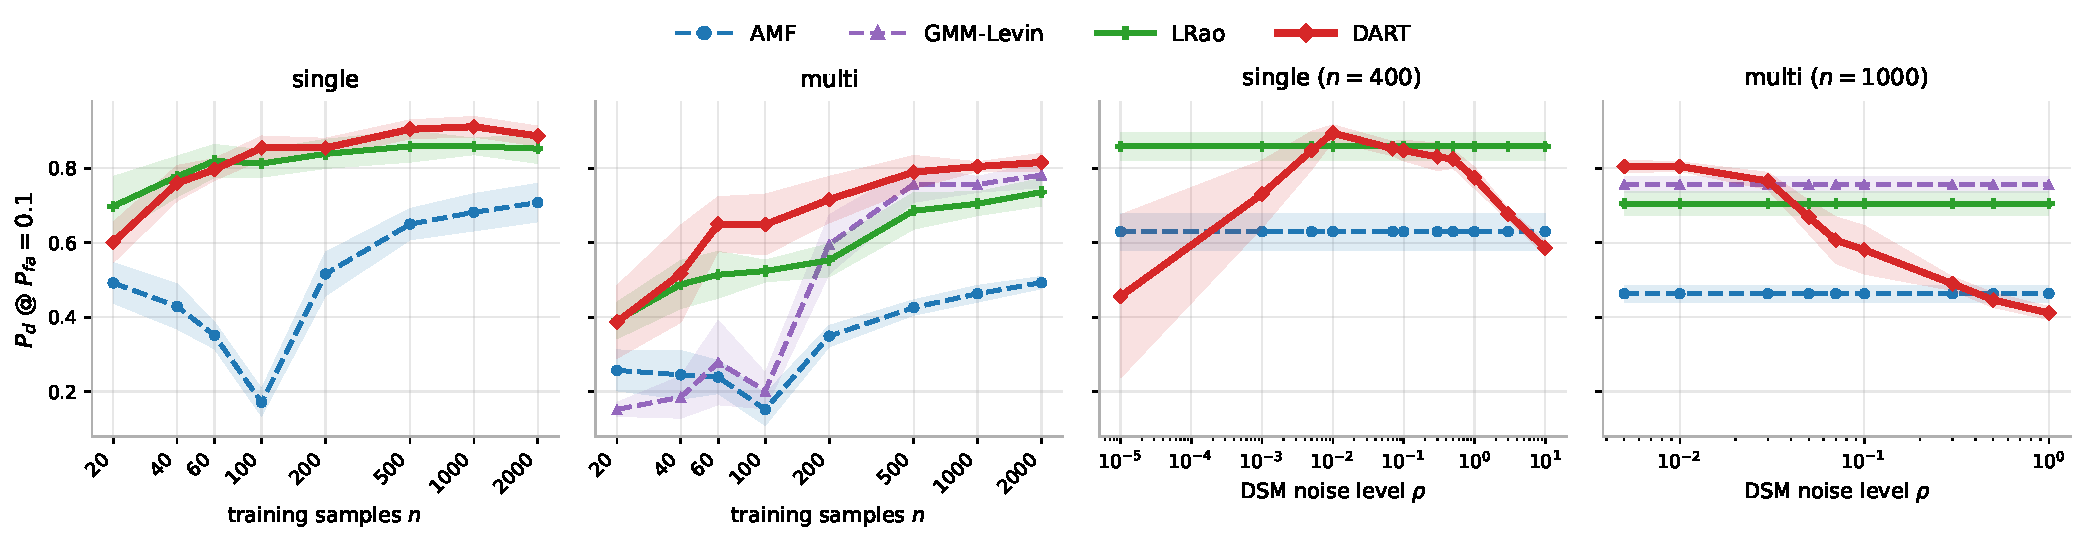
\includegraphics[width=0.55\textwidth, trim=322 238.8 322 9, clip]{figures/iid_grid.pdf}\\[2mm]
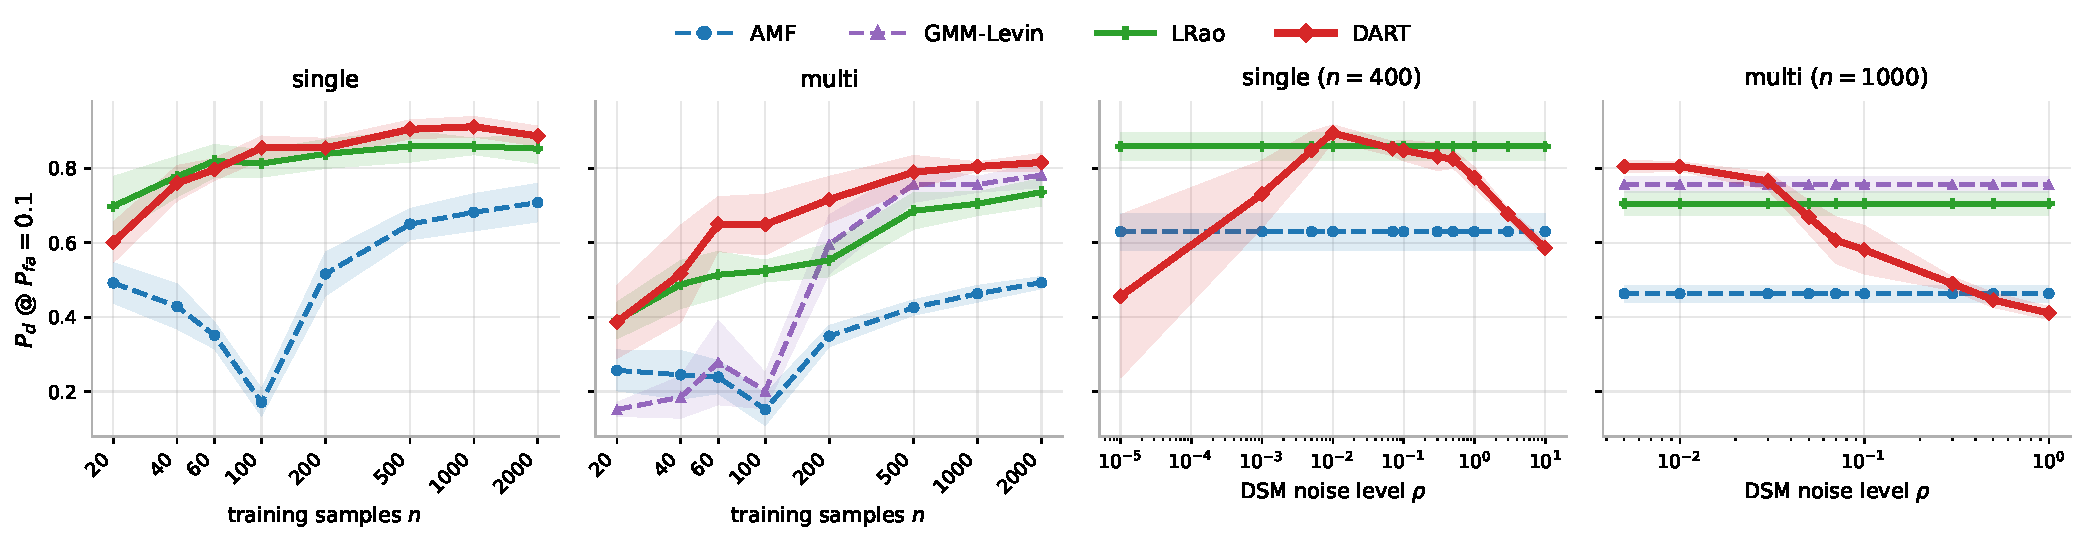
\includegraphics[width=\textwidth, trim=4.8 5.6 487.4 30.4, clip]{figures/iid_grid.pdf}\\[3mm]
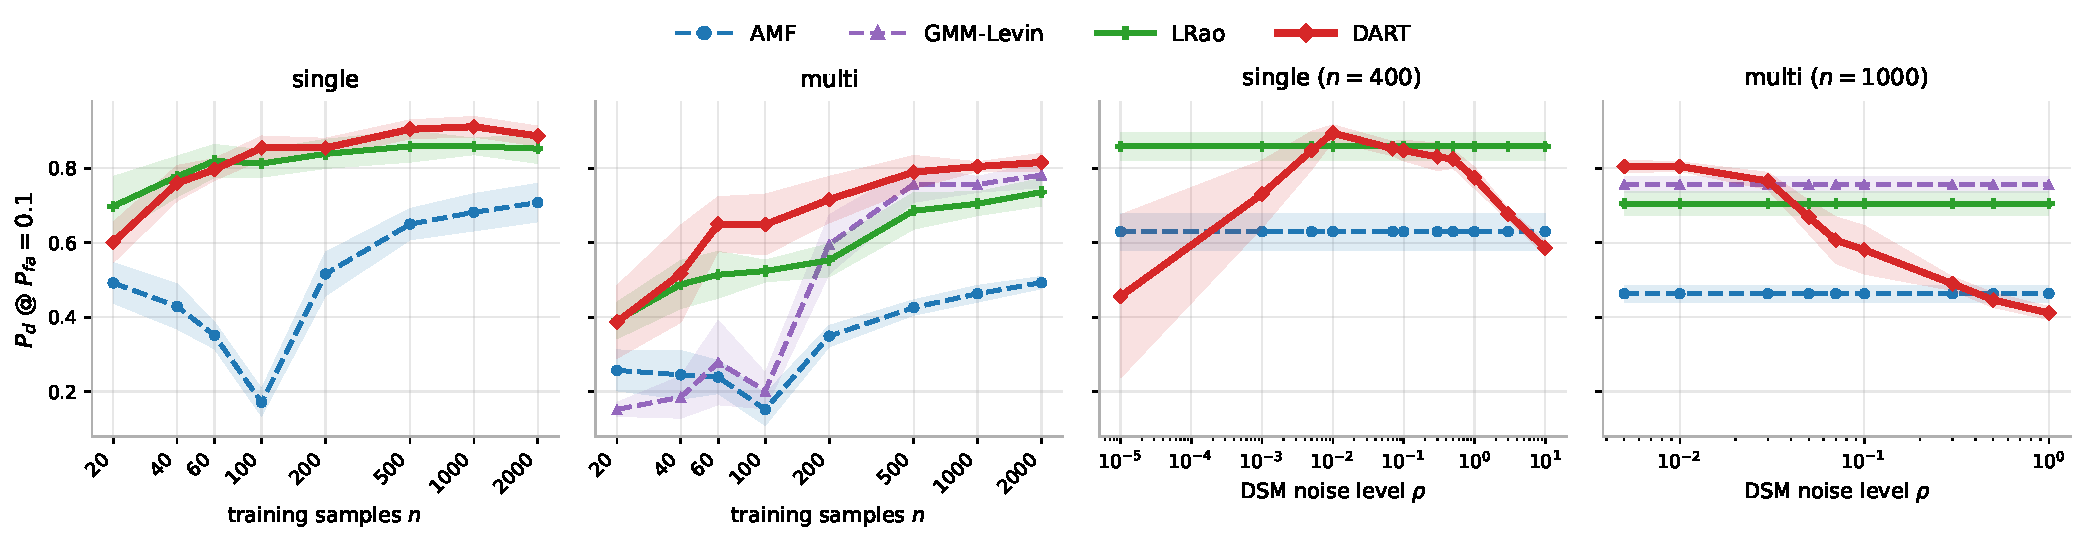
\includegraphics[width=\textwidth, trim=517 5.6 2 30.4, clip]{figures/iid_grid.pdf}
\caption{IID experiments on Pavia University ($5$ seeds, $\pm1\sigma$
bands). \emph{Top row}: $P_d$ at $P_{fa}=0.1$ versus the number of
secondary samples $n$ for the single-class and multi-class backgrounds;
the unregularized AMF collapses near $n\approx d$, where the sample
covariance is rank deficient, whereas the learned detectors are unaffected;
for DART this stability comes from the implicit loading supplied by the DSM
noise. \emph{Bottom row}:
robustness to the DSM noise level $\rho$ at fixed $n$. On the single-class
background, performance is flat over a wide plateau spanning
$\rho\in[5\!\times\!10^{-3},5\!\times\!10^{-1}]$; on the multi-class
background it peaks at small $\rho$ and degrades monotonically as the
blur washes out the mixture structure DART exploits. The operating point
$\rho=0.01$, used in the IID experiments, sits at the optimum in
both cases ($\rho$-independent detectors are drawn as flat references).}
\label{fig:ablation_single}
\label{fig:ablation_multi}
\end{figure}


The first simulation draws the background from a single labeled class, which makes the comparison with the AMF most direct and isolates the regularizing effect of denoising. The first panel of Fig.~\ref{fig:ablation_single} agrees with the Gaussian special case of Section~\ref{sec:special}: the AMF degrades sharply as $n$ approaches the ambient dimension, whereas the implicitly loaded DART is unaffected. LRao is the most effective detector at the smallest sample sizes, and DART leads beyond roughly one hundred samples.

The second simulation combines pixels from six labeled classes into a proportionally mixed background, shifting the emphasis from small-sample stability to the expressive power of the learned score under model mismatch (second panel). DART leads across nearly the entire range of $n$, as the learned score captures non-Gaussian structure that a single Gaussian cannot represent. LRao is the most effective of the remaining detectors at small and moderate sample sizes, and GMM-Levin, whose parametric mixture is well matched to this background, overtakes it at larger $n$.


\section{Correlated background}
\label{sec:spatial}

We now turn to a more realistic setting and evaluate DARTS on Pavia
University, San Diego I, and Salinas. For each scene, we use spatially disjoint training and test boxes, plant targets under the additive model in $10\%$ of the test pixels, and compare local AMF, GMM-Levin, and LRao against the spatially adapted DARTS ($\lambda=0.1$, with a $7\times 7$
neighborhood and $K=7$ pooled neighbors), together with four recent deep detectors, OS-VAE ~\cite{osvae}, HTD-Net ~\cite{htd-net}, THANTD ~\cite{thantd}, and TSTTD ~\cite{tsttd}, each first validated at its published performance on its own benchmark and then trained with its own recipe from the same prior signature and target-free
secondary pixels.
In our runs these baselines were not competitive in this regime and are
therefore omitted from the tables; we defer their detailed treatment to
future work.
As ablations we vary the two ingredients of DARTS in turn
(Table~\ref{tab:spatial}, lower block): the conditioning of the score, by
inserting the unconditioned DART score into the normalized
statistic~\eqref{eq:local_normalized_rao_vector}, and the shrinkage
$\lambda$ of the local score covariance toward the global one. Removing
both recovers the global DART detector.
LRao is trained as its authors prescribe, with early stopping on a held-out validation cost;
the 20\% validation split leaves it fewer secondary pixels than the other
detectors. We report the area under the ROC curve (AUC), the partial AUC
over false alarm rates below $0.05$ (pAUC$_{0.05}$), the detection rate at
a $0.05$ false alarm rate ($P_d@0.05$), and empirical false alarm rates
$\hat P_{fa}$ at thresholds set from the training background scores.

% Table 1 of the MLSP paper (tab:spatial), verbatim.
\begin{table}[htbp]
\centering
\caption{Spatial detection on the correlated Pavia-U scene ($\theta=0.15$,
5 seeds). $\hat P_{fa}^{\max}$ is the largest per-class false alarm rate at
a threshold set to the empirical $0.05$ upper quantile of the training
background scores; the nominal level is $0.05$. Bold marks the best value
within each block. The ablations vary two ingredients of DARTS
independently: whether the score in
Eq.~\eqref{eq:local_normalized_rao_vector} is conditioned on the
neighboring pixels, and the shrinkage $\lambda$ of the local score
covariance toward the global one in
Eq.~\eqref{eq:shrunk_local_fisher}. A dash in the $\lambda$ column
indicates that no local score normalization is applied.}
\label{tab:spatial}
\small
\setlength{\tabcolsep}{5pt}
\renewcommand{\arraystretch}{1.15}
\begin{tabular}{@{}lc ccc c@{}}
\toprule
 & & \multicolumn{3}{c}{Detection} & Calibration\\
\cmidrule(lr){3-5}\cmidrule(l){6-6}
Detector & $\lambda$ & pAUC$_{0.05}$ & AUC & $P_d@0.05$ & $\hat P_{fa}^{\max}$\\
\midrule
DARTS      & 0.1 & \textbf{0.556} & \textbf{0.926} & \textbf{0.730} & \textbf{0.088}\\
\addlinespace[2pt]
AMF        & --  & 0.238 & 0.786 & 0.346 & 0.103\\
GMM-Levin  & --  & 0.129 & 0.773 & 0.229 & 0.455\\
LRao       & --  & 0.137 & 0.713 & 0.220 & 0.761\\
\midrule
\multicolumn{6}{@{}l}{\emph{Ablations --- score conditioning and shrinkage $\lambda$:}}\\
\addlinespace[1pt]
\quad conditioned            & 0.9 & \textbf{0.533} & \textbf{0.925} & \textbf{0.728} & 0.066\\
\quad conditioned            & 1.0 & 0.525 & 0.924 & 0.726 & 0.062\\
\addlinespace[2pt]
\quad unconditioned          & 0.1 & 0.304 & 0.846 & 0.453 & 0.038\\
\quad unconditioned          & 0.9 & 0.311 & 0.846 & 0.443 & \textbf{0.019}\\
\quad unconditioned, no norm.\ & --  & 0.153 & 0.750 & 0.254 & 0.060\\
\bottomrule
\end{tabular}
\end{table}



On Pavia, DARTS attains the highest pAUC, AUC and $P_d$ among the methods
considered, and its largest per class false alarm rate is the closest to
the nominal level. The baselines rank lower, and under a single global
threshold their per class rates depart further from the nominal level.

The ablations isolate the contribution of each ingredient. Local
normalization is valuable on its own: inserting the unconditioned score
into the normalized statistic improves detection substantially over the raw
global statistic. Most of this gain persists when the local score
covariance is shrunk toward the global one, which suggests that the removal
of the local score mean accounts for much of the effect. Normalization
alone, however, is not sufficient. The unconditioned score remains well
below DARTS at matched $\lambda$, which indicates that the benefit of the
neighborhood lies in conditioning the learned score rather than in
correcting it after training. The value of $\lambda$ has only a minor
effect on detection and mainly governs the worst class false alarm rate.


% Table 2 of the MLSP paper (tab:sandiego), verbatim.  The paper sets it as
% a two-column table*; here the two scenes are stacked as two blocks so the
% table fits the A4 text width without shrinking.
\begin{table}[htbp]
\centering
\caption{Spatial detection at a common target amplitude $\theta=0.03$
(5 seeds): San Diego I with the real aircraft signature, Salinas with the
brocoli-green-weeds signature. DARTS uses local moment normalization
($\lambda=0.1$), AMF estimates its mean and covariance in a sliding window,
while GMM-Levin and LRao use their global statistics.}
\label{tab:sandiego}
\small
\setlength{\tabcolsep}{6pt}
\renewcommand{\arraystretch}{1.15}
\begin{tabular}{@{}l c cccc@{}}
\toprule
Detector & $\lambda$ & pAUC$_{0.05}$ & AUC & $P_d$@0.05 & $\hat P_{fa}$\\
\midrule
\multicolumn{6}{@{}l}{\emph{San Diego I}}\\
\addlinespace[1pt]
DARTS       & 0.1 & \textbf{0.634} & \textbf{0.956} & \textbf{0.791} & \textbf{0.020}\\
AMF         & --  & 0.361 & 0.919 & 0.607 & 0.054\\
GMM-Levin   & --  & 0.275 & 0.777 & 0.397 & 0.025\\
LRao        & --  & 0.177 & 0.776 & 0.276 & 0.041\\
\midrule
\multicolumn{6}{@{}l}{\emph{Salinas}}\\
\addlinespace[1pt]
DARTS       & 0.1 & 0.766 & \textbf{0.972} & \textbf{0.882} & \textbf{0.009}\\
AMF         & --  & \textbf{0.769} & 0.968 & 0.866 & 0.055\\
GMM-Levin   & --  & 0.038 & 0.864 & 0.062 & 0.132\\
LRao        & --  & 0.169 & 0.845 & 0.237 & 0.084\\
\bottomrule
\end{tabular}
\end{table}


Table~\ref{tab:sandiego} reports the same protocol on San Diego I and
Salinas. The target amplitude is reduced to $\theta=0.03$, where the scenes
remain challenging; at larger amplitudes the detectors saturate.
The results follow the same pattern, with DARTS comparing favorably on
both scenes. The local AMF is the strongest baseline here, and on Salinas,
whose large homogeneous fields are well matched to a local Gaussian model,
it comes close to DARTS. Amplitude sweeps and the reuse of a single learned
background model across additional target signatures are demonstrated in the
accompanying code repository.